\documentclass[../piano-di-progetto.tex]{subfiles}

\begin{document}

\section{Analisi dei rischi}
Durane lo sviluppo di un progetto complesso, è possibile incorrere in problemi che potrebbero essere evitati tramite un processo preliminare di analisi dei rischi. Con l'obiettivo di prevenire ed evitare queste evenienze, è stata effettuata un’attenta analisi dei principali fattori di rischio svolgendo i seguenti passi:

\begin{itemize}
    \item \textbf{Identificazione dei rischi}: individuazione dei possibili fattori di rischio che potrebbero rallentare o bloccare il normale svolgersi del progetto;
    \item \textbf{Analisi dei rischi}: valutazione delle probabilità di occorrenza del rischio, valutazione delle ripercussioni sul progetto e, infine, assegnazione di un indice di grado del rischio;
    \item \textbf{Pianificazione di controllo}: definizione della metodologia per evitare di incorrere nei rischi individuati e come procedere nell'eventualità in cui non sia possibile evitarne alcuni;
    \item \textbf{Monitoraggio dei rischi}: monitoraggio continuo al fine di rilevare quanto prima l'incombere di un rischio con l'obiettivo di poterlo evitare oppure limitare le ripercussioni sullo svolgersi del progetto.
\end{itemize}

\subsection{Valutazione}
Viene utilizzato il sistema a matrice di valutazione dei rischi. Ad ogni rischio viene associato un indice di gravità, ottenuto considerando la probabilità che tale rischio possa accedere e l'impatto che esso avrà sullo svolgersi del progetto. Questo indice può assumere i seguenti valori:
\begin{itemize}
    \item Basso;
    \item Medio;
    \item Alto;
    \item Critico;
\end{itemize}
\begin{figure}[H]
	\centering
	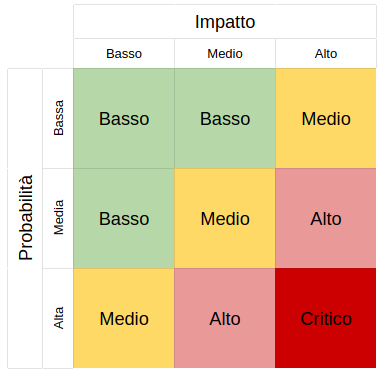
\includegraphics[width=10cm]{img/matrice-rischio.png}
	\caption{Matrice dell'indice di gravità del rischio}
	\label{fig:matrice-rischio}
  \end{figure}

\subsection{Classificazione}
Ad ogni rischio viene assegnato un codice univoco affinché possa essere identificato e facilmente riconoscibile. La struttura del codice identificativo è la seguente: \\
\texttt{RK-[Categoria]-[ID]-[Indice di gravità]} \\
I tre campi assumono i seguenti valori:
\begin{itemize}
    \item \textbf{Categoria}:
        \begin{itemize}
            \item \textbf{O}: organizzativo;
            \item \textbf{P}: personale;
            \item \textbf{T}: tecnologico.
        \end{itemize}
    \item \textbf{ID}: rappresenta un numero intero incrementale all'interno della categoria;
    \item \textbf{Indice di gravità}: valore ottenuto dalla matrice in figura \ref{fig:matrice-rischio} con la seguente associazione:
        \begin{itemize}
            \item \textbf{1}: Basso;
            \item \textbf{2}: Medio;
            \item \textbf{3}: Alto;
            \item \textbf{4}: Critico;
        \end{itemize}
\end{itemize}

\subsection{Possibili rischi}
    \begin{longtable}{cccc}
        \caption{Tabella dei rischi} \\
        \hline
        \textbf{Codice} & \textbf{Descrizione} & \textbf{Identificazione} \\
        \hline
        \endfirsthead
        \multicolumn{3}{c}%
        {\tablename\ \thetable\ -- \textit{Continuazione della pagina precendente}} \\
        \hline
        \textbf{Codice} & \textbf{Descrizione} & \textbf{Identificazione} \\
        \hline
        \endhead
        \hline \multicolumn{3}{r}{\textit{Continua alla prossima pagina}} \\
        \endfoot
        \hline
        \endlastfoot
        Codice e nome                                                                              & Descrizione                                                                                                                                                                                                & \multicolumn{2}{l}{Identificazione}                                                                                                                                                                           \\
        \begin{tabular}[c]{@{}l@{}}RK-P1-4\\ \\ Inesperienza \\ tecnologica\end{tabular}           & \begin{tabular}[c]{@{}l@{}}Non tutti i componenti del gruppo hanno le conoscenze \\ sulle tecnologie richieste dal proponente\end{tabular}                                                                 & \multicolumn{2}{l}{\begin{tabular}[c]{@{}l@{}}Il Responsabile parlerà \\ periodicamente con ogni \\ membro del gruppo per capire \\ le conoscenze del singolo \\ individuo\end{tabular}}                      \\
        Piano di contingenza                                                                       & \multicolumn{3}{l}{\begin{tabular}[c]{@{}l@{}}Ogni componente si impegna a sanare le proprie mancanze in modo da poter lavorare in\\ autonomia sui compiti a lui assegnati\end{tabular}}                                                                                                                                                                                                                                   \\
        \hline
        \begin{tabular}[c]{@{}l@{}}RK-P2-3\\ \\ Inesperienza \\ gestionale\end{tabular}            & \begin{tabular}[c]{@{}l@{}}Nessun membro del gruppo si è mai trovato nelle \\ condizioni di lavorare ad un progetto di dimensioni \\ così elevate\end{tabular}                                             & \multicolumn{2}{l}{\begin{tabular}[c]{@{}l@{}}Il Responsabile avrà il compito\\ di assicurarsi che ogni membro \\ del gruppo abbia compreso \\ pienamente il ruolo e compiti a \\ lui assegnati\end{tabular}} \\
        Piano di contingenza                                                                       & \multicolumn{3}{l}{\begin{tabular}[c]{@{}l@{}}Ogni componente si impegna a studiare in modo autonomo i compiti e doveri associati \\ ad ogni ruolo e informare il Responsabile in caso di perplessità\end{tabular}}                                                                                                                                                                                                        \\
            \hline
        \begin{tabular}[c]{@{}l@{}}RK-P3-3\\ \\ Impegni \\ accademici\end{tabular}                 & \begin{tabular}[c]{@{}l@{}}Alcuni membri del gruppo potrebbero non essere \\ sempre disponibili per continuare lo sviluppo \\ del progetto a causa di impegni accademici\end{tabular}                      & \multicolumn{2}{l}{\begin{tabular}[c]{@{}l@{}}Il Responsabile verificherà \\ periodicamente lo stato degli \\ impegni accademici dei singoli \\ componenti\end{tabular}}                                      \\
        Piano di contingenza                                                                       & \multicolumn{3}{l}{\begin{tabular}[c]{@{}l@{}}Sarà compito dei singoli individui programmare gli impegni accademici in modo tale\\ che non interferiscano con lo svolgersi del progetto. Inoltre, il Responsabile a \\ conoscenza degli impegni accademici dei singoli, assegnerà compiti compatibili \\ con essi\end{tabular}}                                                                                            \\
            \hline
        \begin{tabular}[c]{@{}l@{}}RK-P4-2\\ \\ Impegni \\ personali\end{tabular}                  & \begin{tabular}[c]{@{}l@{}}Alcuni membri del gruppo potrebbero essere \\ indisponibili a causa di impegni personali\end{tabular}                                                                           & \multicolumn{2}{l}{\begin{tabular}[c]{@{}l@{}}I membri del gruppo dovranno \\ segnalare al Responsabile \\ eventuali indisponibilità\end{tabular}}                                                            \\
        Piano di contingenza                                                                       & \multicolumn{3}{l}{\begin{tabular}[c]{@{}l@{}}In caso di ritardi, sarà compito del Responsabile valutare una riassegnazione dei \\ compiti in modo da poter rispettare i tempi prestabiliti\end{tabular}}                                                                                                                                                                                                                  \\
            \hline
        \begin{tabular}[c]{@{}l@{}}RK-P5-2\\ \\ Abbandono \\ del gruppo\end{tabular}               & \begin{tabular}[c]{@{}l@{}}Per motivi personali, un membro del gruppo \\ potrebbe decidere di abbandonare lo sviluppo\end{tabular}                                                                         & \multicolumn{2}{l}{\begin{tabular}[c]{@{}l@{}}Il componente che intende \\ lasciare lo sviluppo deve \\ informare il prima possibile il\\ resto del gruppo\end{tabular}}                                      \\
        Piano di contingenza                                                                       & \multicolumn{3}{l}{\begin{tabular}[c]{@{}l@{}}Si valuterà se l'abbandono del gruppo da parte del componente potrà diventare \\ solo una temporaneo congedo\end{tabular}}                                                                                                                                                                                                                                                   \\
            \hline
        \begin{tabular}[c]{@{}l@{}}RK-O1-3\\ \\ Calcolo dei \\ costi e \\ tempistiche\end{tabular} & \begin{tabular}[c]{@{}l@{}}A causa delle dimensioni molto elevate del progetto \\ e dalla inesperienza dei membri del gruppo, le \\ stime dei tempi e dei costi potrebbe risultare incoerente\end{tabular} & \multicolumn{2}{l}{\begin{tabular}[c]{@{}l@{}}Ogni membro ha il compito di \\ informare il Responsabile nel \\ caso in cui il proprio compito \\ stia superando le ore previste\end{tabular}}                 \\
        Piano di contingenza                                                                       & \multicolumn{3}{l}{\begin{tabular}[c]{@{}l@{}}Se le ore effettive richieste da un certo compito stanno per superare le ore \\ preventivate, verrà considerata una ripartizione di quest'ultimo\end{tabular}}                                                                                                                                                                                                               \\
            \hline
        \begin{tabular}[c]{@{}l@{}}RK-O2-2\\ \\ Conflitti interni\end{tabular}                     & \begin{tabular}[c]{@{}l@{}}Potrebbero verificarsi situazioni di tensione \\ tra due o più membri del gruppo\end{tabular}                                                                                   & \multicolumn{2}{l}{\begin{tabular}[c]{@{}l@{}}Appena questa situazione si \\ verifica, è compito dei membri\\  coinvolti mettere al corrente il\\  resto del gruppo\end{tabular}}                             \\
        Piano di contingenza                                                                       & \multicolumn{3}{l}{\begin{tabular}[c]{@{}l@{}}Il Responsabile, o un componente non coinvolto, assumerà l'incarico di \\ mediatore per risolvere la situazione\end{tabular}}                                                                                                                                                                                                                                                \\
            \hline
        \begin{tabular}[c]{@{}l@{}}RK-O4-2\\ \\ Comunicazione \\ con il \\ proponente\end{tabular} & \begin{tabular}[c]{@{}l@{}}Il proponente potrebbe non essere disponibile a causa \\ di impegni lavorativi\end{tabular}                                                                                     & \multicolumn{2}{l}{\begin{tabular}[c]{@{}l@{}}Sin dal primo colloqui di \\ cercherà di capire le \\ disponibilità del proponente\end{tabular}}                                                                \\
        Piano di contingenza                                                                       & \multicolumn{3}{l}{\begin{tabular}[c]{@{}l@{}}Il gruppo cercherà di chiarire quanti più dubbi possibili durante ogni colloquio \\ preparando in anticipo una lista di domande\end{tabular}}                                                                                                                                                                                                                                \\
            \hline
        \begin{tabular}[c]{@{}l@{}}RK-T1-2\\ \\ Problemi software \\ e hardware\end{tabular}       & \begin{tabular}[c]{@{}l@{}}Qualcuno potrebbe riscontrare problemi software \\ o hardware all'interno del computer, non potendo \\ proseguire nell'immediato con lo sviluppo del progetto\end{tabular}      & \multicolumn{2}{l}{\begin{tabular}[c]{@{}l@{}}Ogni componente dovrà \\ segnalare tempestivamente \\ il problema riscontrato \\ tramite un dispositivo non \\ affetto da guasti\end{tabular}}                  \\
    Piano di contingenza                                                                       & \multicolumn{3}{l}{\begin{tabular}[c]{@{}l@{}}Nel caso la riparazione non potesse essere portata a termine in tempi molto brevi, il singolo \\ dovrà utilizzare un computer sostitutivo per continuare lo sviluppo. Nell'evenienza in cui il \\ componente non avesse a disposizione nessun dispositivo allora il Responsabile dovrà \\ procedere alla riassegnazione dei compiti\end{tabular}}                           
    \end{longtable}
\end{document}